\documentclass[12pt]{article}
\usepackage{times}
\usepackage[english]{babel}
\usepackage[utf8x]{inputenc}
\usepackage[colorinlistoftodos]{todonotes}
\usepackage[margin=1in]{geometry}
\usepackage{graphicx}
\usepackage{epstopdf}
\usepackage{cite}
\usepackage{listings}
\usepackage{dtklogos}
\usepackage{wrapfig}
\usepackage{subfigure}
\usepackage{amsmath}
\usepackage{amsthm}
\usepackage{amssymb}
\usepackage{amscd}
\usepackage{caption}
\usepackage{etoolbox}
\usepackage{fancyhdr}
\usepackage{stackengine}
\usepackage[export]{adjustbox}
\patchcmd{\thebibliography}{\section*{\refname}}{}{}{}
\usepackage[document]{ragged2e}    %This causes text to left align
\usepackage[colorlinks=true, linkcolor=black,citecolor=black,urlcolor=blue]{hyperref}
\bibliographystyle{IEEEtran}
\extrafloats{100}
\DeclareGraphicsRule{.tif}{png}{.png}{`convert #1 `dirname #1`/`basename #1 .tif`.png}

\title{MCHE 357: Lab 7}

\begin{document}
\lefthyphenmin3
\righthyphenmin4
% \pretolerance=2000
% \tolerance=500 
% \emergencystretch=10pt
%\raggedright     %Stops LaTeX from automatically hyphenating the right margin to fit better
%Combine this with \usepackage[document]{ragged2e} to get a text align left similar to natural MS Word


%-------------------------------------------------------------
%Start of Paper
%-------------------------------------------------------------

%%%%%%%%%%%%%%%%%%%%%%%%%%%%%%%%%%%%%%%%%%%%%%%%%%%%%%
%%%%%%%%%%%%%%%%%%%%%%% TITLE PAGE %%%%%%%%%%%%%%%%%%%%%%%%
%%%%%%%%%%%%%%%%%%%%%%%%%%%%%%%%%%%%%%%%%%%%%%%%%%%%%%

\begin{titlepage}

\newcommand{\HRule}{\rule{\linewidth}{0.5mm}} % Defines a new command for the horizontal lines, change thickness here

\center % Center everything on the page
 
%----------------------------------------------------------------------------------------
%	Heading Section
%----------------------------------------------------------------------------------------

\textsc{\LARGE University of Louisiana at Lafayette}\\[1.5cm] % Name of your university/college
\textsc{\Large Measurements and Instrumentation}\\[0.5cm] % Major heading such as course name
\textsc{\large MCHE 357}\\[0.5cm] % Minor heading such as course title

%----------------------------------------------------------------------------------------
%	Title Section
%----------------------------------------------------------------------------------------

\HRule \\[0.4cm]
{ \huge \bfseries Lab 7}\\[0.4cm] % Title of your document
\HRule \\[1.5cm]
 
%----------------------------------------------------------------------------------------
%	Author Section
%----------------------------------------------------------------------------------------

\begin{minipage}{0.4\textwidth}
\begin{flushleft} \large
\emph{Author:}\\
\textsc{Matthew J. Begneaud} \\% Your name
\end{flushleft}
\end{minipage}
~
\begin{minipage}{0.4\textwidth}
\begin{flushright} \large
\emph{Professor:} \\
\textsc{Dr. Mostafa A. Elsayed} % Supervisor's Name
\end{flushright}
\end{minipage}\\[1.5cm]

% If you don't want a supervisor, uncomment the two lines below and remove the section above
%\Large \emph{Author:}\\
%John \textsc{Smith}\\[3cm] % Your name

%----------------------------------------------------------------------------------------
%	Date Section
%----------------------------------------------------------------------------------------

{\textsc{\large \today}}\\[0.5cm] % Date, change the \today to a set date if you want to be precise


%----------------------------------------------------------------------------------------
%	Group Section
%----------------------------------------------------------------------------------------
\textsc{\large Group:}\\[0.1cm]
\textsc{Ronald Kisor}\\
\textsc{Chandler Lagarde}\\
\textsc{Somto Umeokafor}
\\[0.5cm]

%----------------------------------------------------------------------------------------
%	Logo Section
%----------------------------------------------------------------------------------------


\includegraphics[width=5in]{UL_logo.jpg}\\[1cm] % Include a department/university logo - this will require the graphicx package
 
%----------------------------------------------------------------------------------------

\vfill % Fill the rest of the page with whitespace

\end{titlepage}

%%%%%%%%%%%%%%%%%%%%%%%%%%%%%%%%%%%%%%%%%%%%%%%%%%%%%%
%%%%%%%%%%%%%%%%%%%%%%% TABLE OF CONTENTS %%%%%%%%%%%%%%%%%%%
%%%%%%%%%%%%%%%%%%%%%%%%%%%%%%%%%%%%%%%%%%%%%%%%%%%%%%

\tableofcontents

\listoffigures

\bigskip


\section*{\fontsize{12}{12}\selectfont \large List of Symbols}
\addcontentsline{toc}{section}{List of Symbols} % Add for each section
None




\newpage

%%%%%%%%%%%%%%%%%%%%%%%%%%%%%%%%%%%%%%%%%%%%%%%%%%%%%%
%%%%%%%%%%%%%%%%%%%%%%% REPORT %%%%%%%%%%%%%%%%%%%%%%%%%%
%%%%%%%%%%%%%%%%%%%%%%%%%%%%%%%%%%%%%%%%%%%%%%%%%%%%%%


\section*{\fontsize{12}{12}\selectfont \large Introduction}
\addcontentsline{toc}{section}{Introduction} % Add for each section
This lab consisted of learning to use an Arduino, a simple microcontroller used often by hobbyists and even some professionals to gather data or control small electronic systems. In this lab, the board was used to blink an LED at a fixed rate, at a rate determined by a potentiometer, and writing voltages out to pins.


\section*{\fontsize{12}{12}\selectfont \large Theory}
\addcontentsline{toc}{section}{Theory} % Add for each section

Digital systems are by nature only capable of generating a fixed voltage, meaning that the voltage output is either on or off. However, systems often require that voltages between off and on are required. Digital systems can recreate analog systems in this way by use of a method called pulse-width-modulation (PWM). This method times extremely quick pulses of voltage such that the average voltage of the signal over time amounts to a desired voltage level. 
\bigskip

An Arduino microcontroller can also read a signal, or voltage input. This allows the board to read a potentiometer, for example. This can allow a user to change system parameters with a potentiometer without changing the program on the mirocontroller.
\bigskip


\section*{\fontsize{12}{12}\selectfont \large Procedure \& Analysis}
\addcontentsline{toc}{section}{Procedure \& Analysis} % Add for each section

The first program uploaded to the Arduino board was used to toggle an LED on or off every second. This was done by sending a voltage to the LED for one second, and then turning the voltage output off for one second. This program is simply repeated indefinitely. The physical setup for this program is shown in Figure 1.
\bigskip

The second program uploaded to the Arduino board was used to toggle an LED on or off with a frequency dependent on the reading from a potentiometer. This was done by reading the voltage that was coming back from the potentiometer. This value was then mapped to a time for the microcontroller to delay before toggling the LED. The physical setup used for this program is shown in Figure 2.
\bigskip

The third program uploaded to the Arduino board outputted a voltage to a pin which was then read with a multimeter. This program utilized PWM in order to write to a pin any desired voltage between off and on levels. The physical system used for this program, including the multimeter reading, is shown in Figure 3.
\bigskip
 
 \newpage

\begin{figure}[h!] %  figure placement: here, top, bottom, or page
   \centering
   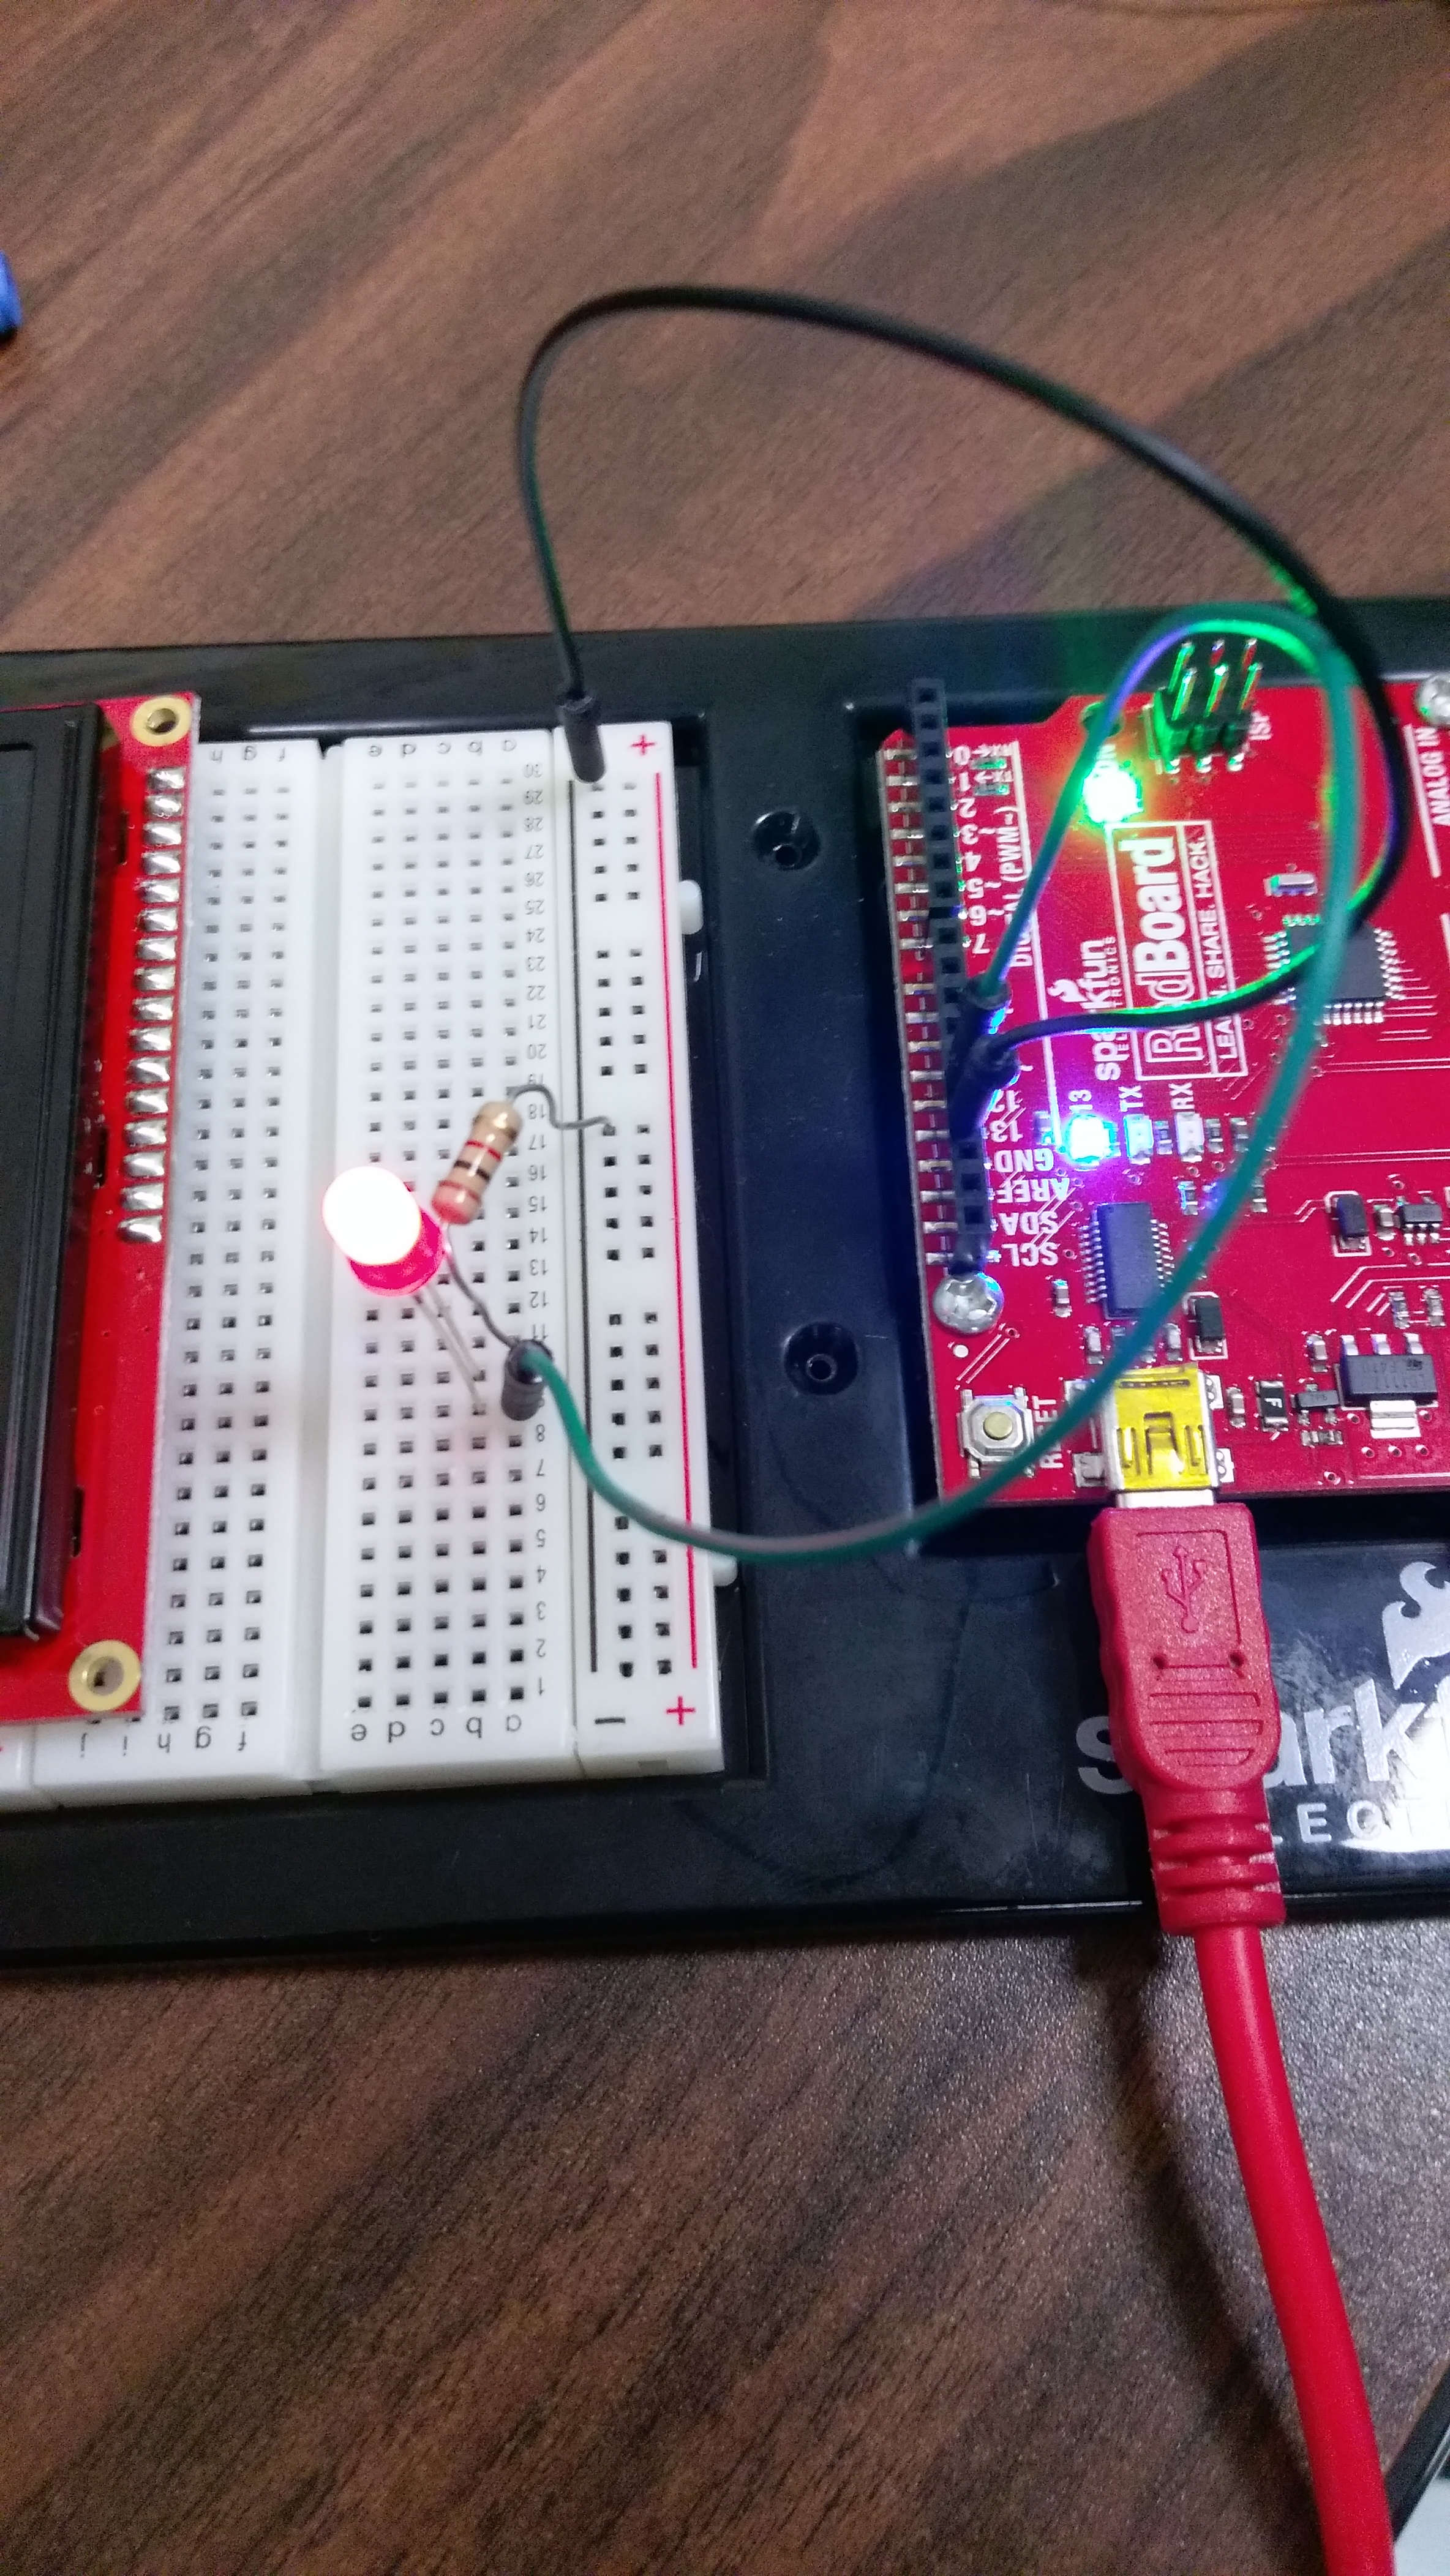
\includegraphics[width=3in, height=3.5in]{blinking_on.jpg} 
   \caption{Blinking LED at Fixed Rate (On)}
   \label{fig:example}
\end{figure}

\begin{figure}[h!] %  figure placement: here, top, bottom, or page
   \centering
   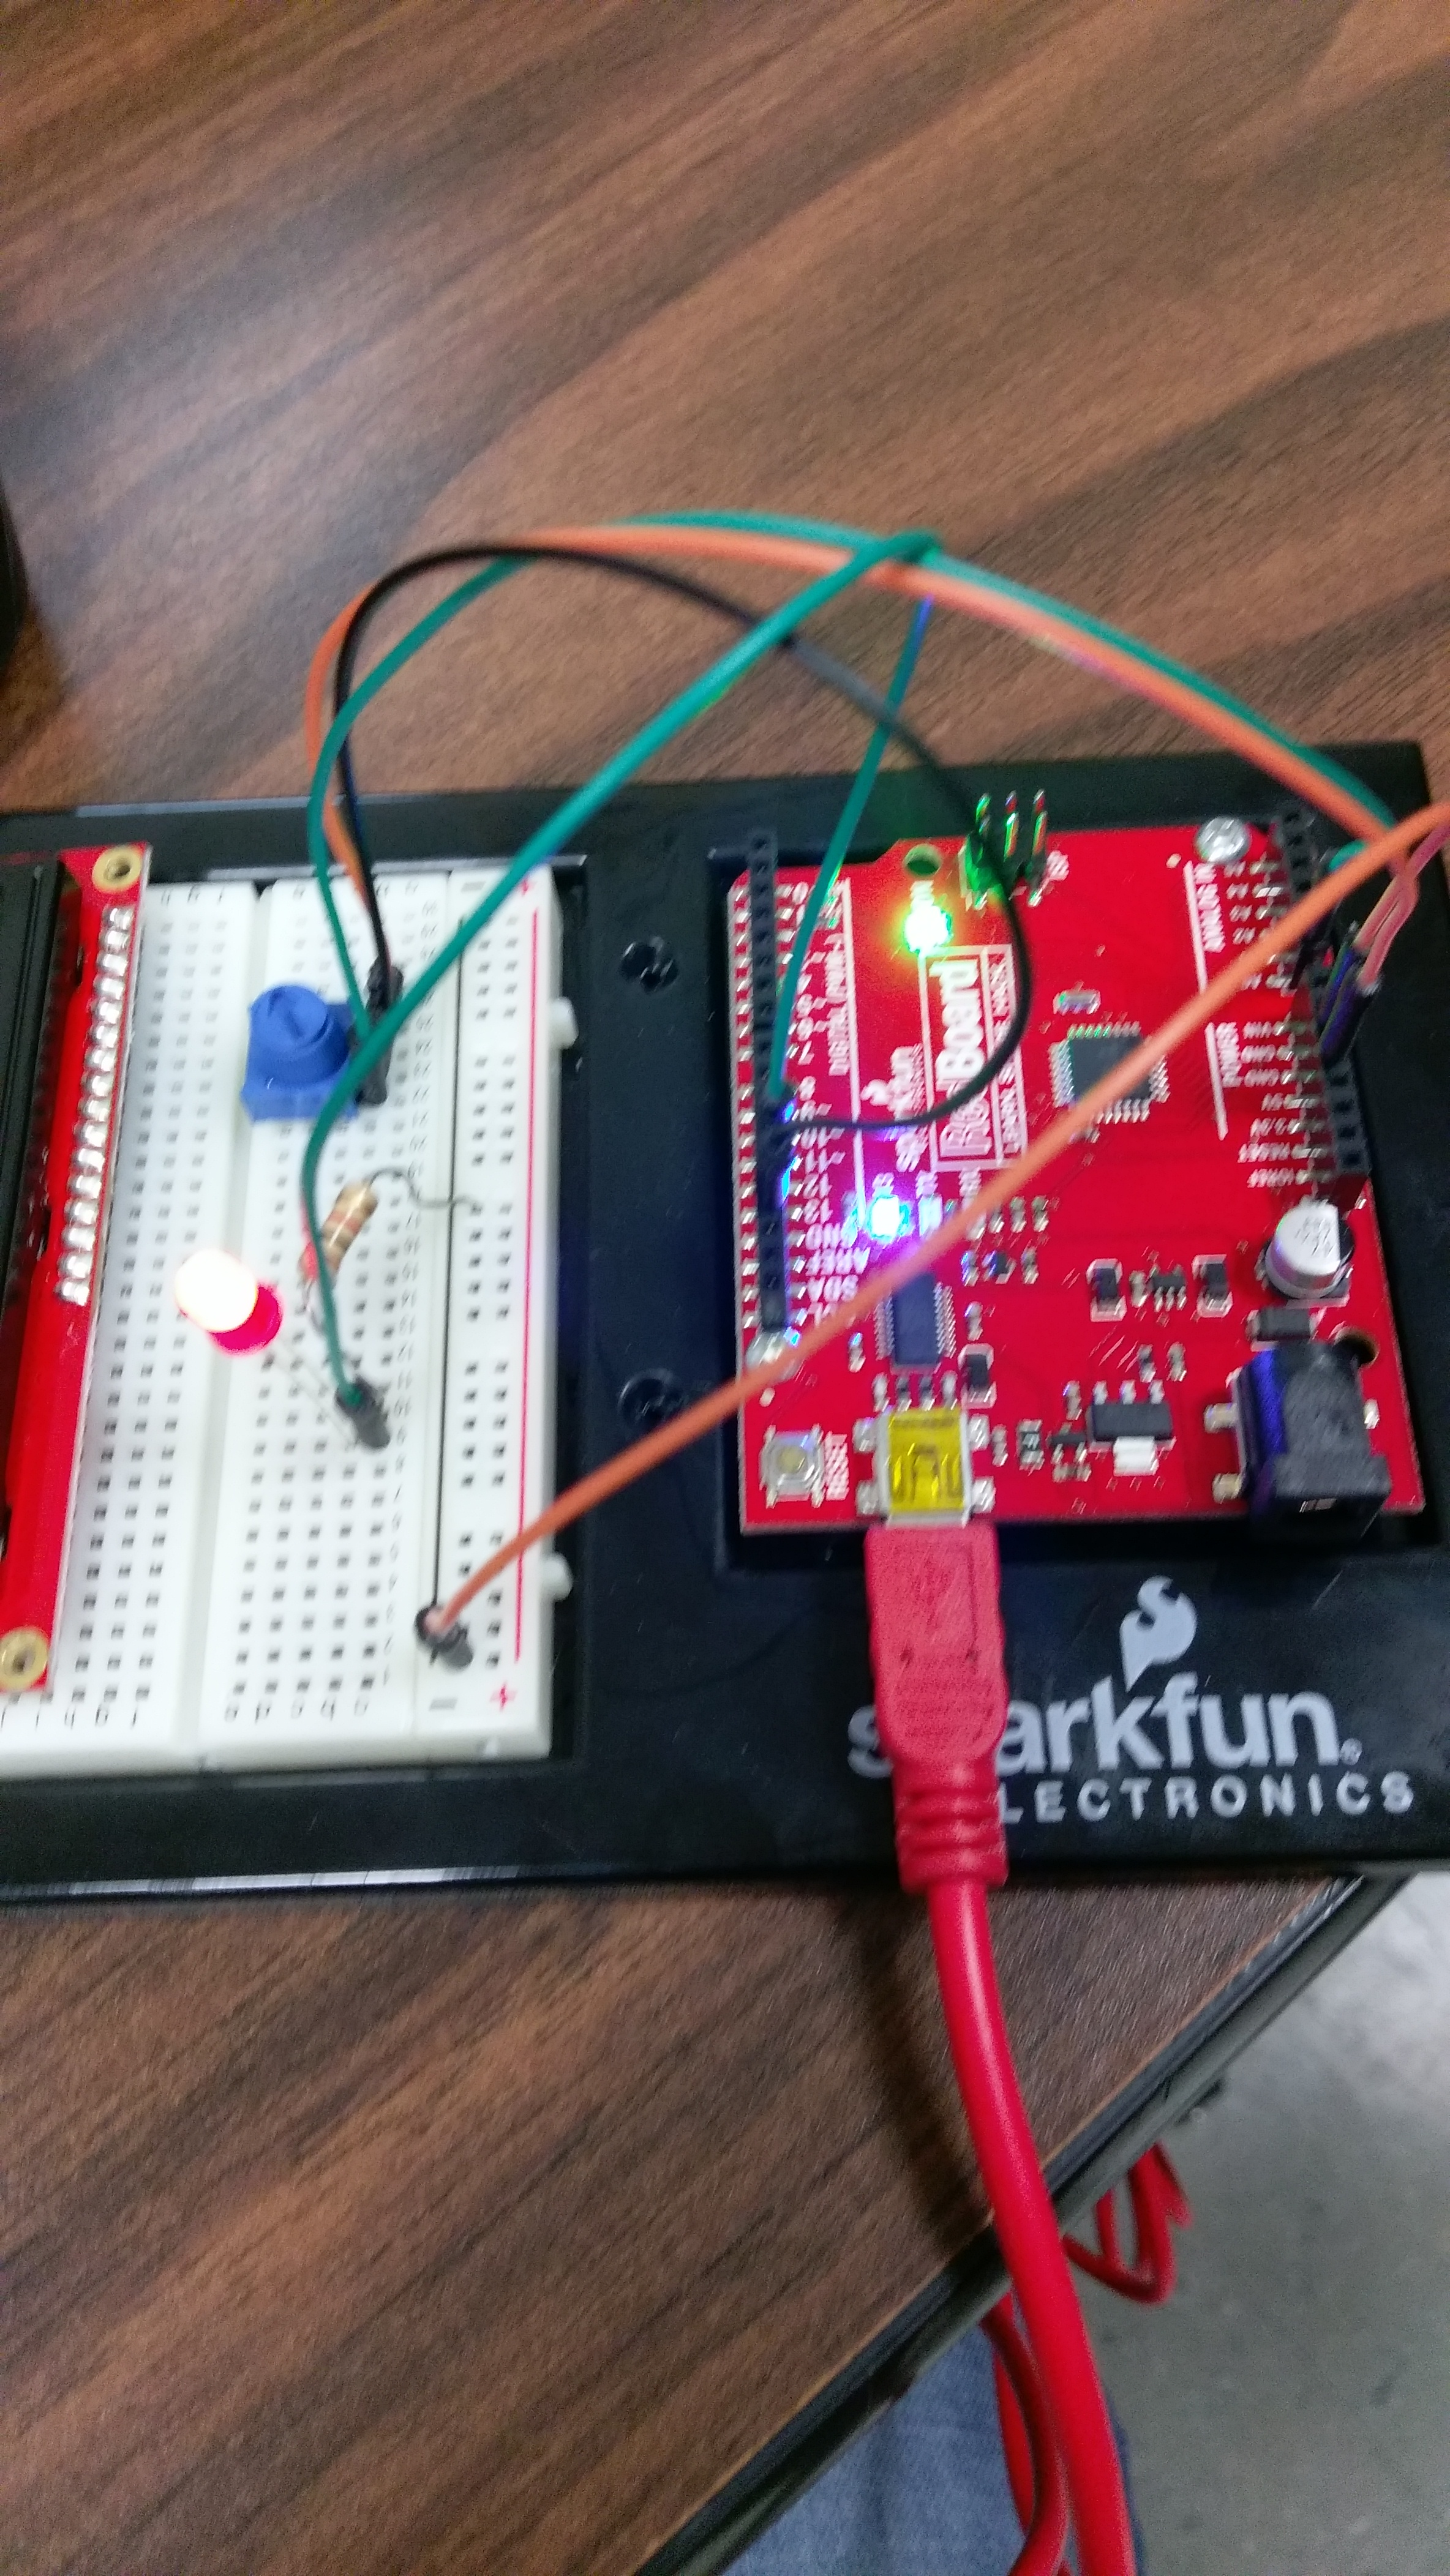
\includegraphics[width=3in, height=3.5in]{blinking_with_pot.jpg} 
   \caption{Blinking LED at Potentiometer Rate (On)}
   \label{fig:example}
\end{figure}

\newpage

\begin{figure}[h!] %  figure placement: here, top, bottom, or page
   \centering
   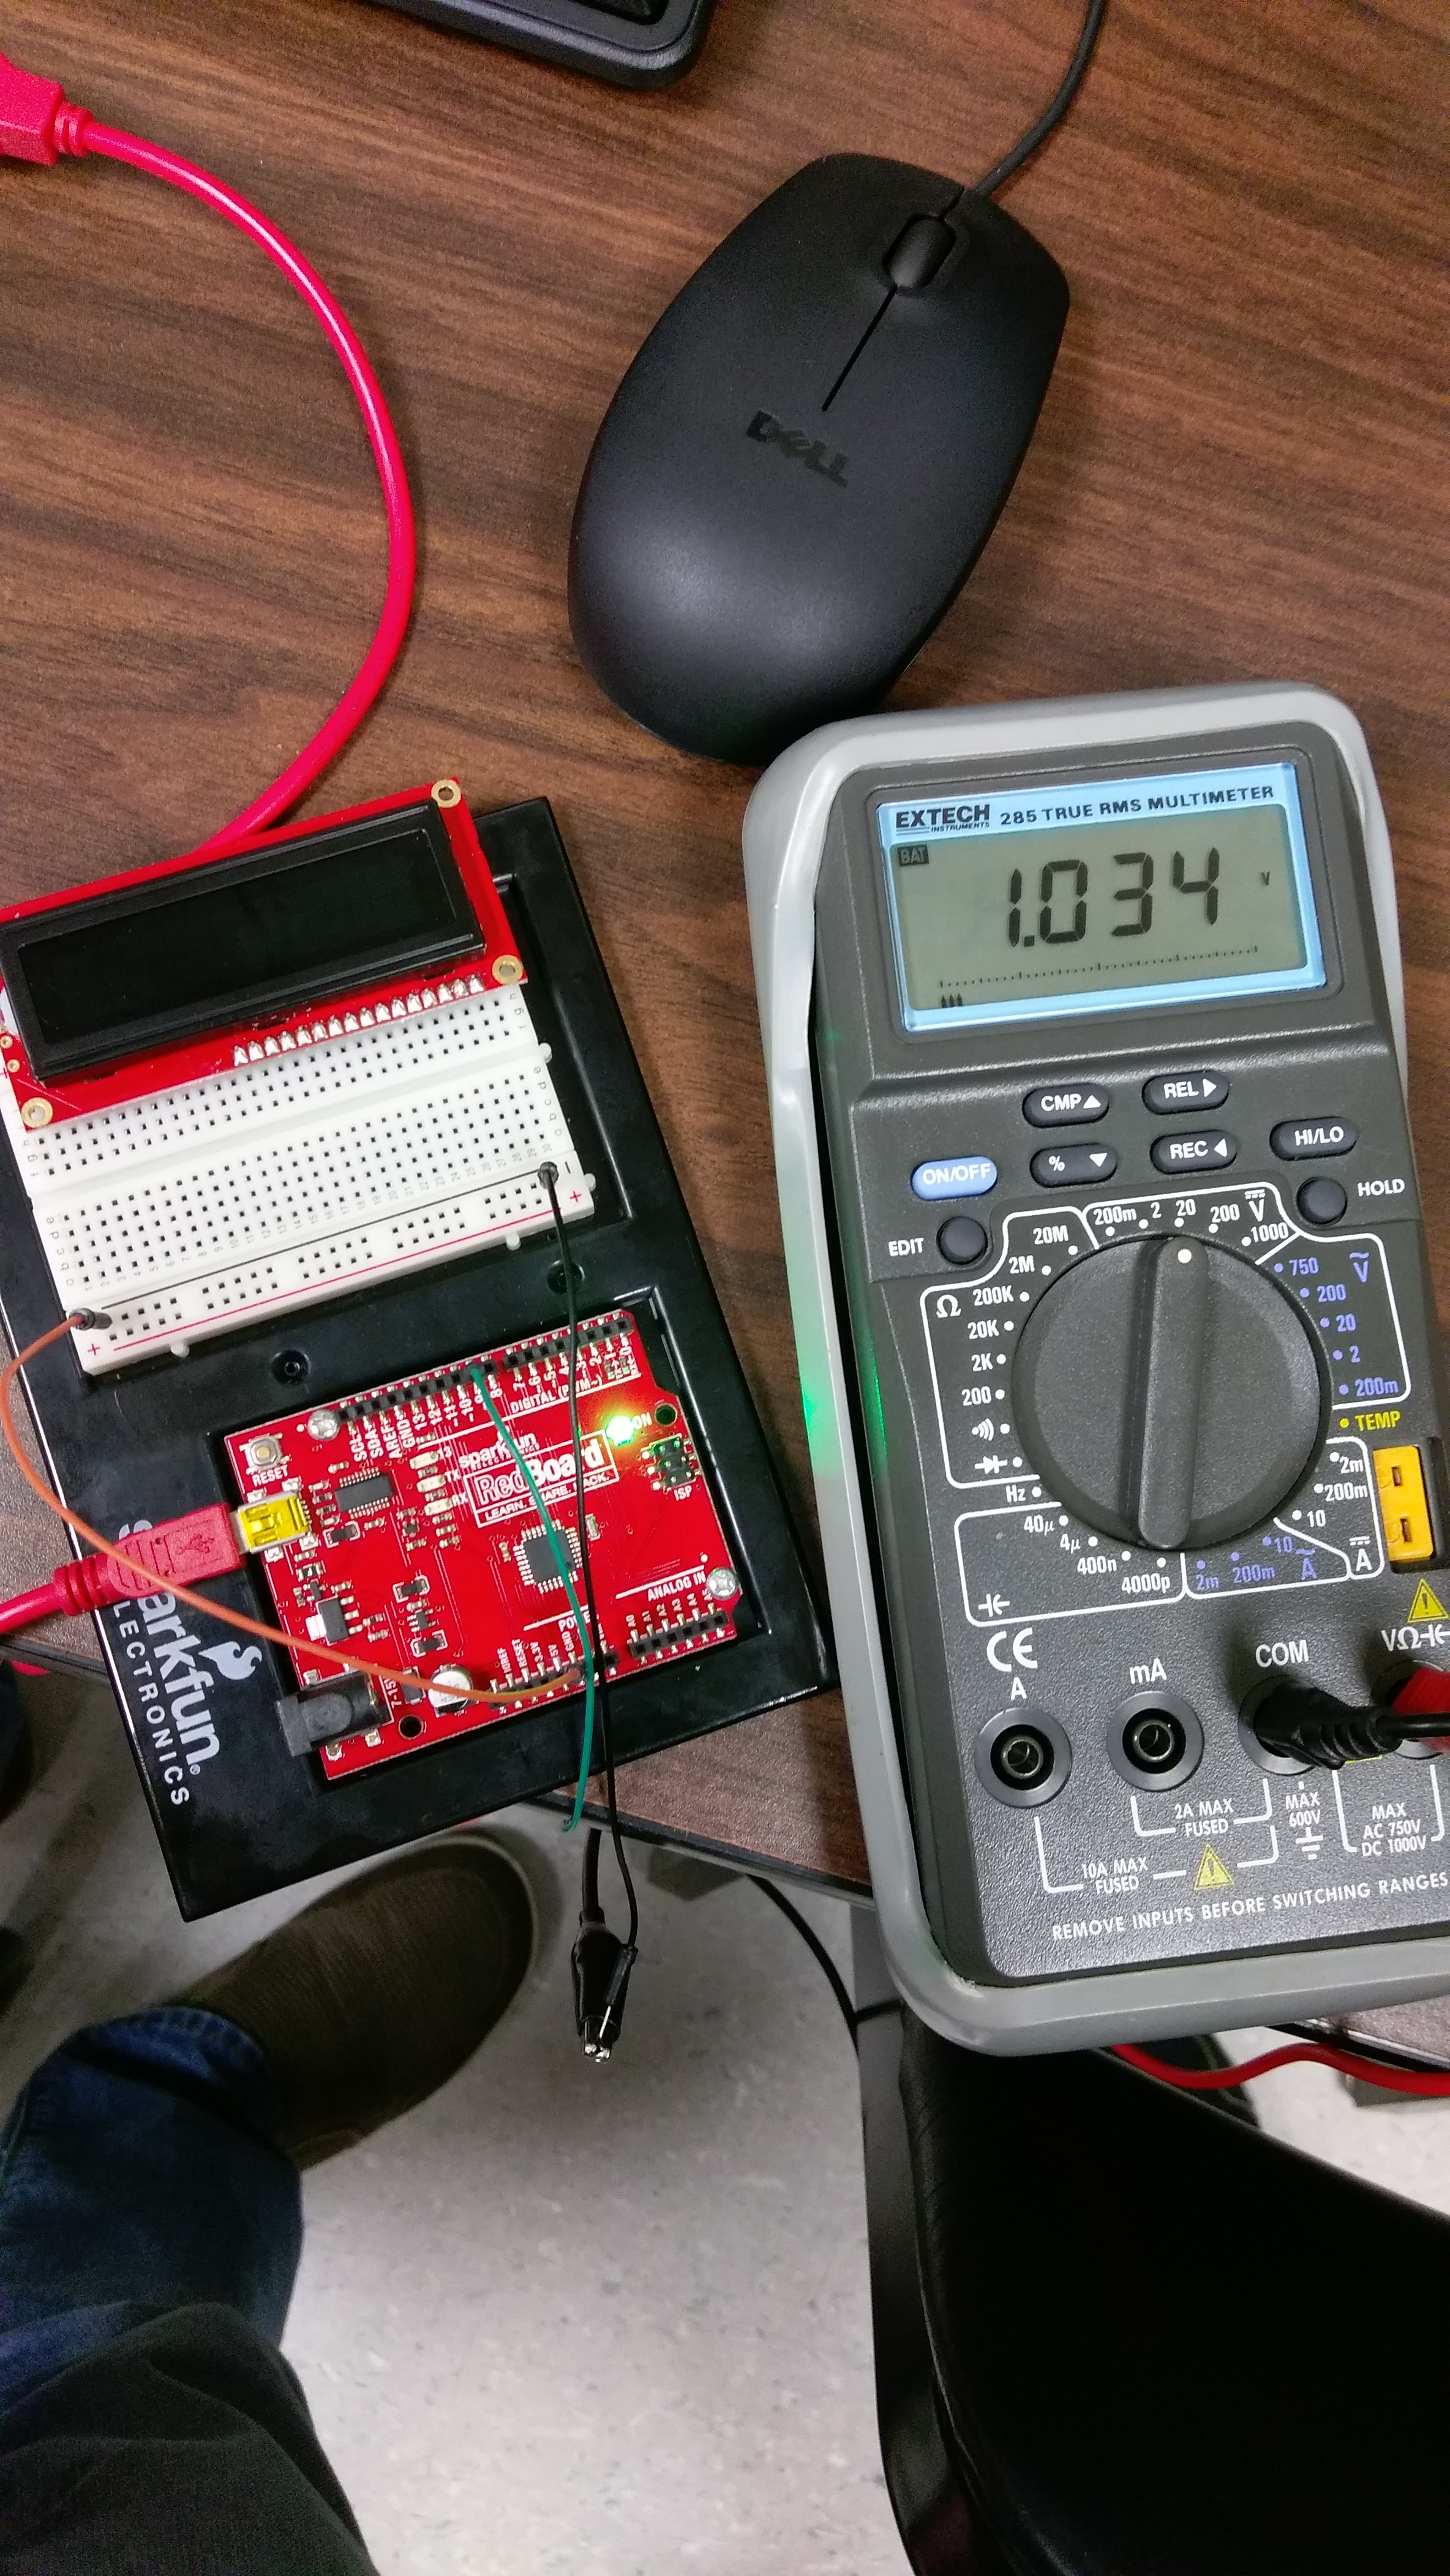
\includegraphics[width=3in, height=4.5in]{read_output.jpg} 
   \caption{Signal Output Reading}
   \label{fig:example}
\end{figure}

\bigskip

\section*{\fontsize{12}{12}\selectfont \large Conclusion}
\addcontentsline{toc}{section}{Conclusion} % Add for each section
The exercises conducted in this lab demonstrated using an Arduino microcontroller. It was shown that while simple, easy to use, and cost efficient, an Arduino board can be a powerful tool for use in engineering experimentation. It is well used to control systems as well as acquire data. It is useful for engineering students to gain experience with microcontrollers, as they are found all throughout industry. 


%\section*{\fontsize{12}{12}\selectfont \large References}

%\begin{thebibliography}{2}
%
%% Example
%%\bibitem{Wagner}
%%Ng, K., Wagner, S.W., Camelio, J., Emblom, W.J. (2010). ?Experimental Analysis of Micro Tube
%%Hydroforming Process.? Transactions of NAMRC of SME, 38, 577-584.
%
%\end{thebibliography}



%\section*{\fontsize{12}{12}\selectfont APPENDIX}

%\begin{table}[h!]
%  \caption{}
%  \includegraphics[width=\linewidth]{table1.png}
%\end{table}




\end{document}







----------------------------Templates-------------------------------

-------------------------Figure-----------------------

\begin{figure}[h!]  
  \centering
    \includegraphics[width=\linewidth]{**file**}
    \caption{Docking Station}
\end{figure}

---------------------------Table-----------------------
\begin{table}[ht]
\caption{Nonlinear Model Results} % title of Table
\centering % used for centering table
\begin{tabular}{c c c c} % centered columns (4 columns)
\hline\hline %inserts double horizontal lines
Case & Method\#1 & Method\#2 & Method\#3 \\ [0.5ex] % inserts table
%heading
\hline % inserts single horizontal line
1 & 50 & 837 & 970 \\ % inserting body of the table
2 & 47 & 877 & 230 \\
3 & 31 & 25 & 415 \\
4 & 35 & 144 & 2356 \\
5 & 45 & 300 & 556 \\ [1ex] % [1ex] adds vertical space
\hline %inserts single line
\end{tabular}
\label{table:nonlin} % is used to refer this table in the text
\end{table}



probably best to insert as an image from excel

\bigskip\\
\begin{table}[h!]
  \caption{}
  \includegraphics[width=\linewidth]{**file**}
\end{table}
\bigskip\\





-----------------------------Equations------------------------
-----------------------------Regular
\begin{equation}
a = b + c
\end{equation}

--------------------------------- Multiline
\begin{multline}
a = b + c + d + e + f
+ g + h + i + j \\
+ k + l + m + n + o
\end{multline}

-------------------------------Citations-------------------------
\bibitem{Author last name}
  Last, First., year of publication,
  article name, book(etc) name, from \\
  link goes here

----------------------------------other-----------------------------

equations:
http://moser-isi.ethz.ch/docs/typeset_equations.pdf

citations:
http://library.missouri.edu/engineering/about/guides/asme
https://www.asme.org/shop/proceedings/conference-publications/references